\section{Auswertung}

Dieses Kapitel präsentiert die Ergebnisse der Evaluation der entwickelten Anwendung im Hinblick auf die in Kapitel \ref{einleitung} formulierten Forschungsfragen.  
Die Auswertung verfolgt das Ziel, die Gebrauchstauglichkeit (Usability), Verständlichkeit sowie die Eignung der Lösung für kollaborative Planungssituationen zu überprüfen.  
Dazu wurden sowohl quantitative Methoden in Form der standardisierten \textit{System Usability Scale} (SUS) als auch qualitative Verfahren wie Beobachtungen, Freitextfeedback und ein praxisnaher Feldtest eingesetzt.  
Diese methodische Kombination ermöglicht es, einerseits messbare, vergleichbare Kennzahlen zu erheben und andererseits detaillierte Einblicke in die Nutzererfahrung und potenzielle Verbesserungspotenziale zu gewinnen.



\subsection{Zielsetzung der Auswertung}

Die Evaluation der entwickelten Anwendung verfolgt das Ziel, ihre Gebrauchstauglichkeit, Verständlichkeit und Eignung für kollaborative Nutzung zu untersuchen. Dabei stehen insbesondere die drei formulierten Forschungsfragen im Fokus:
\begin{itemize}
    \item Wie intuitiv ist die Nutzung für Laien?
    \item Wie verständlich und zugänglich ist die Oberfläche trotz Funktionsvielfalt?
    \item Wie wird die Lösung in realen Anwendungsszenarien wahrgenommen?
\end{itemize}

\subsection{Durchführung und Methodik}

Die Evaluation erfolgte in Form von nutzerzentrierten Usability-Tests mit Teilnehmenden aus der relevanten Zielgruppe. Die Testpersonen bearbeiteten ein Szenario mit mehreren Aufgaben zur Raumgestaltung mithilfe des Infrarotstifts.


Der Ablauf umfasste:
\begin{itemize}
    \item eine kurze Einführung in das System,
    \item die eigenständige Nutzung der Anwendung,
    \item die Beantwortung der System Usability Scale (SUS),
    \item eine Freitext-Rückmeldung sowie
    \item eine passive Beobachtung durch das Projektteam.
\end{itemize}

Zusätzlich wurden Feldtests mit dem Kunden (SCDH) durchgeführt. Dabei wurde das System in realistischen Anwendungsszenarien erprobt und im Anschluss strukturierte Interviews durchgeführt.

\begin{figure}[H]
    \begin{minipage}{0.48\textwidth}
    \centering
    \frame{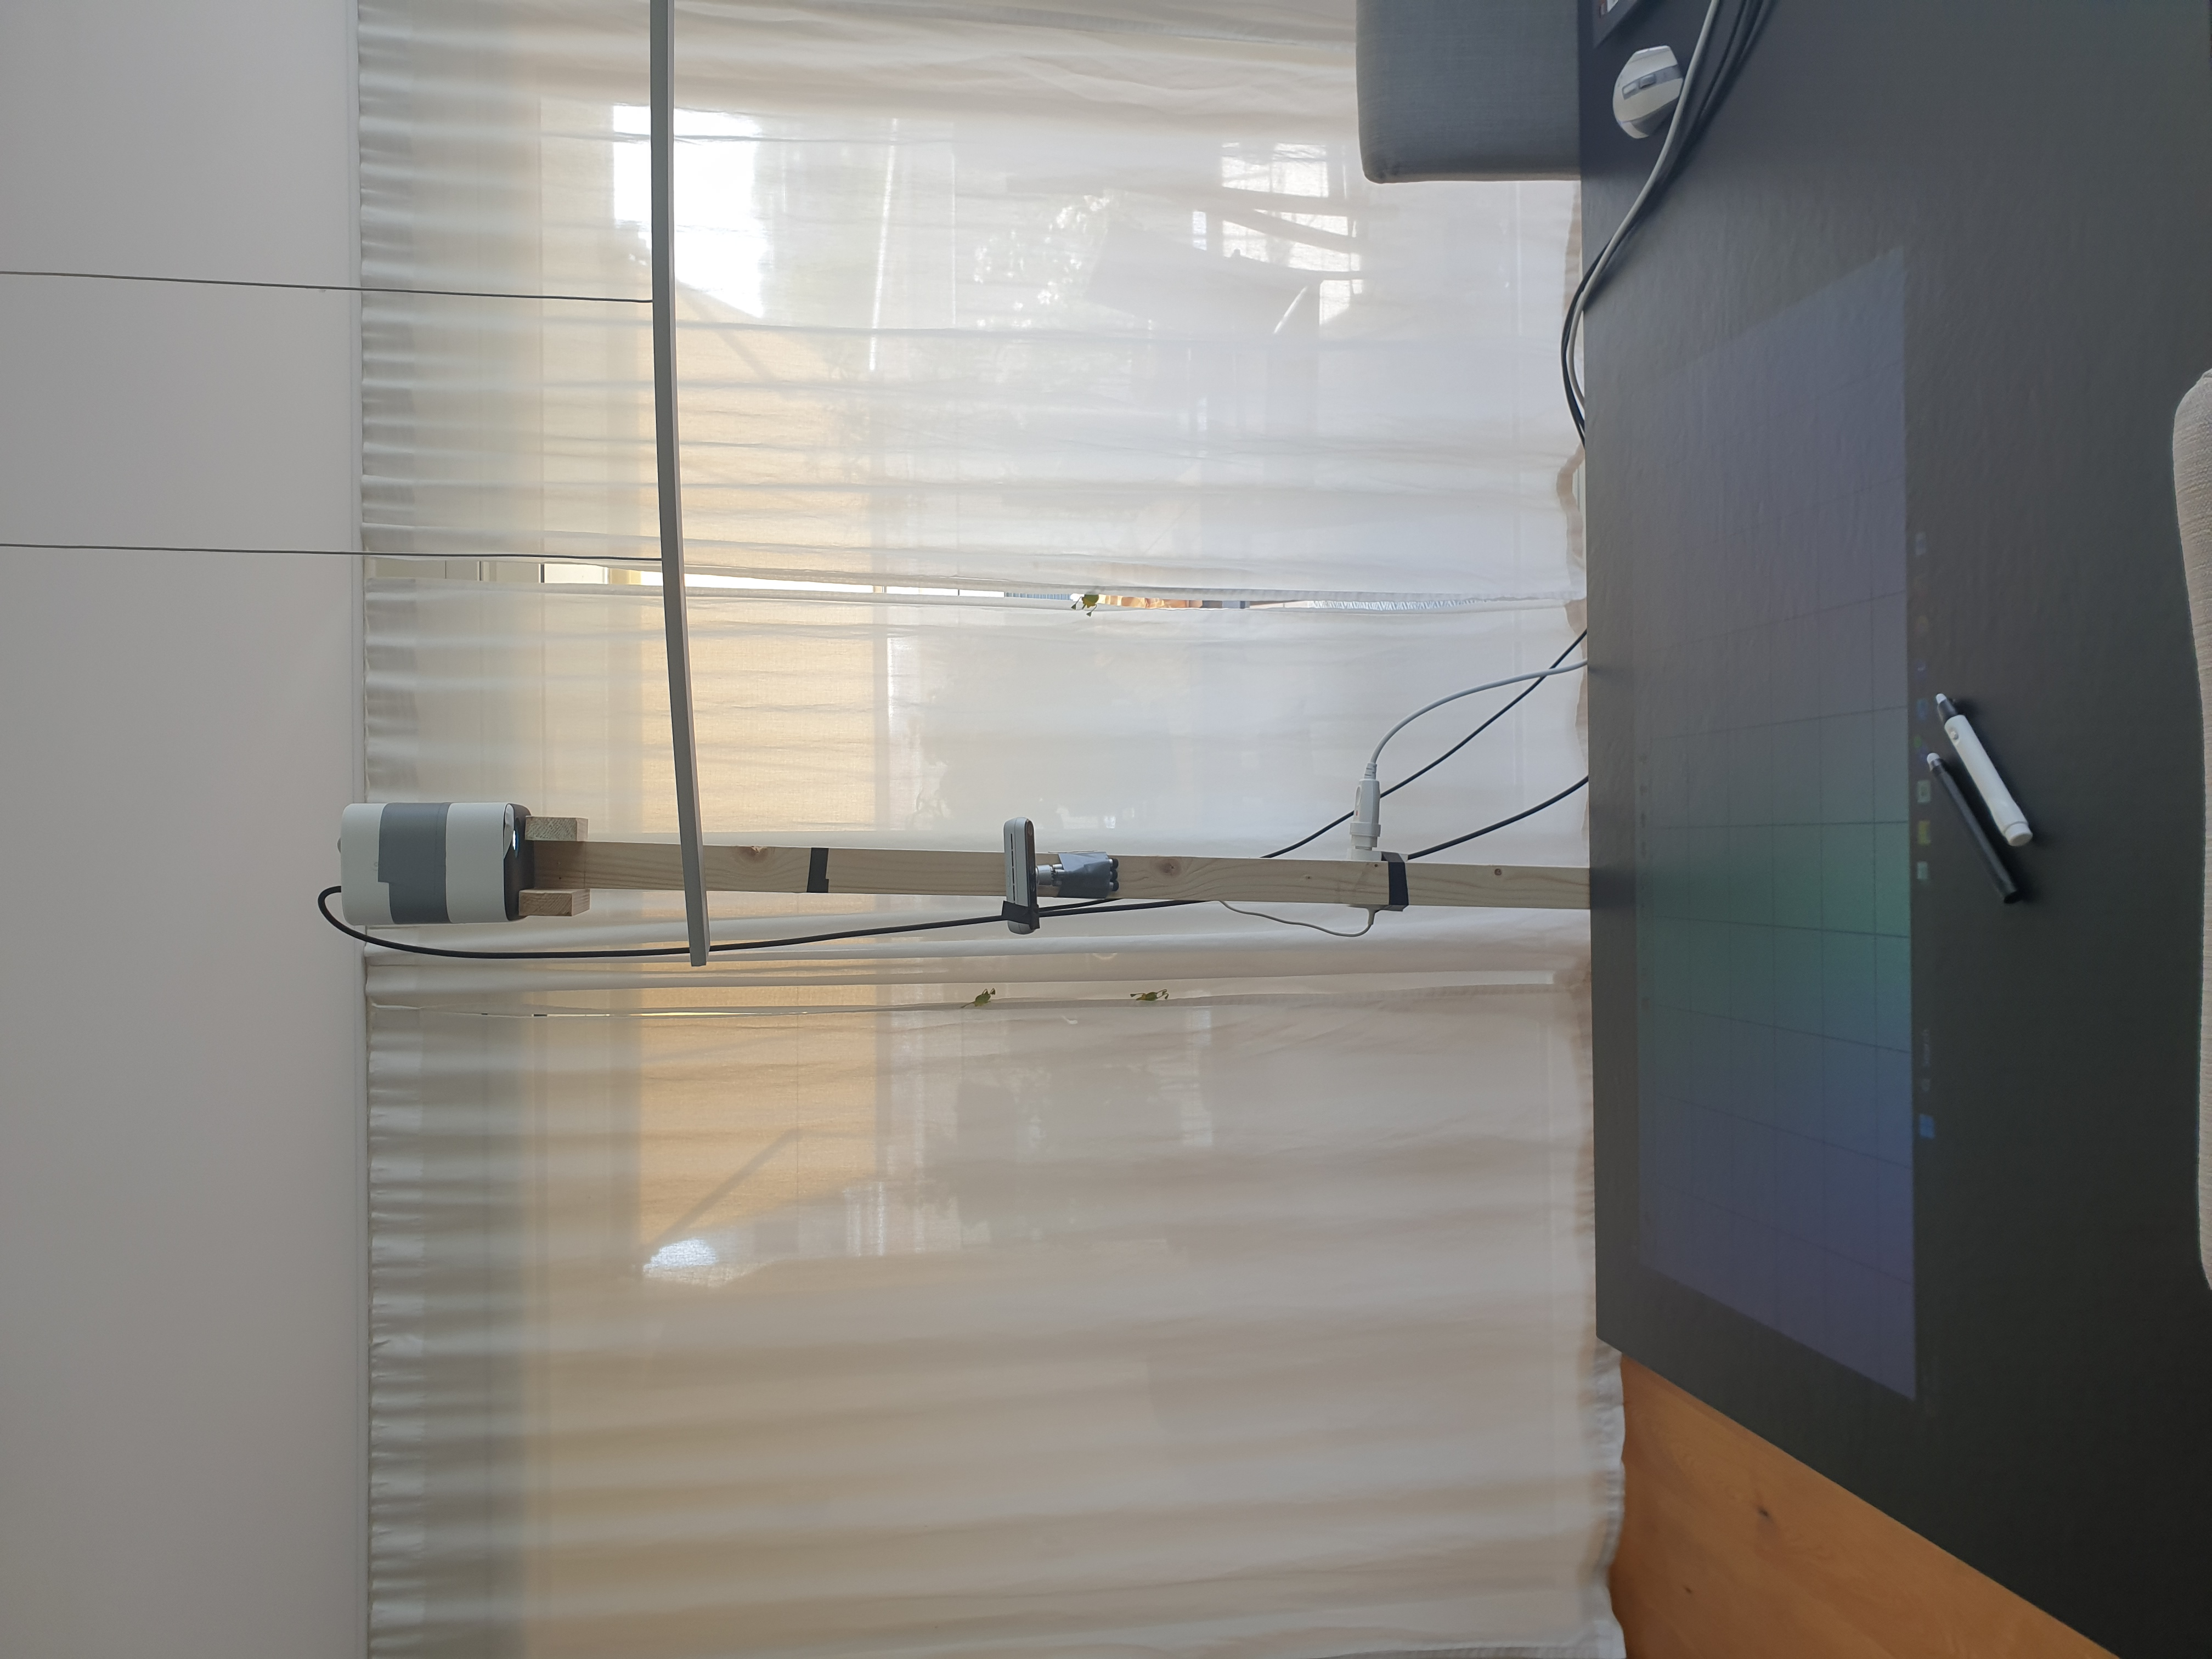
\includegraphics[width=0.7\linewidth, angle=-90]{graphics/sus_setup_1.jpg}}
    \caption{Testaufbau mit Projektion und IR-Stift (SUS)}
    \label{Fig:Data1}
  \end{minipage}
  \hfill
  \begin{minipage}{0.48\textwidth}
    \centering
    \frame{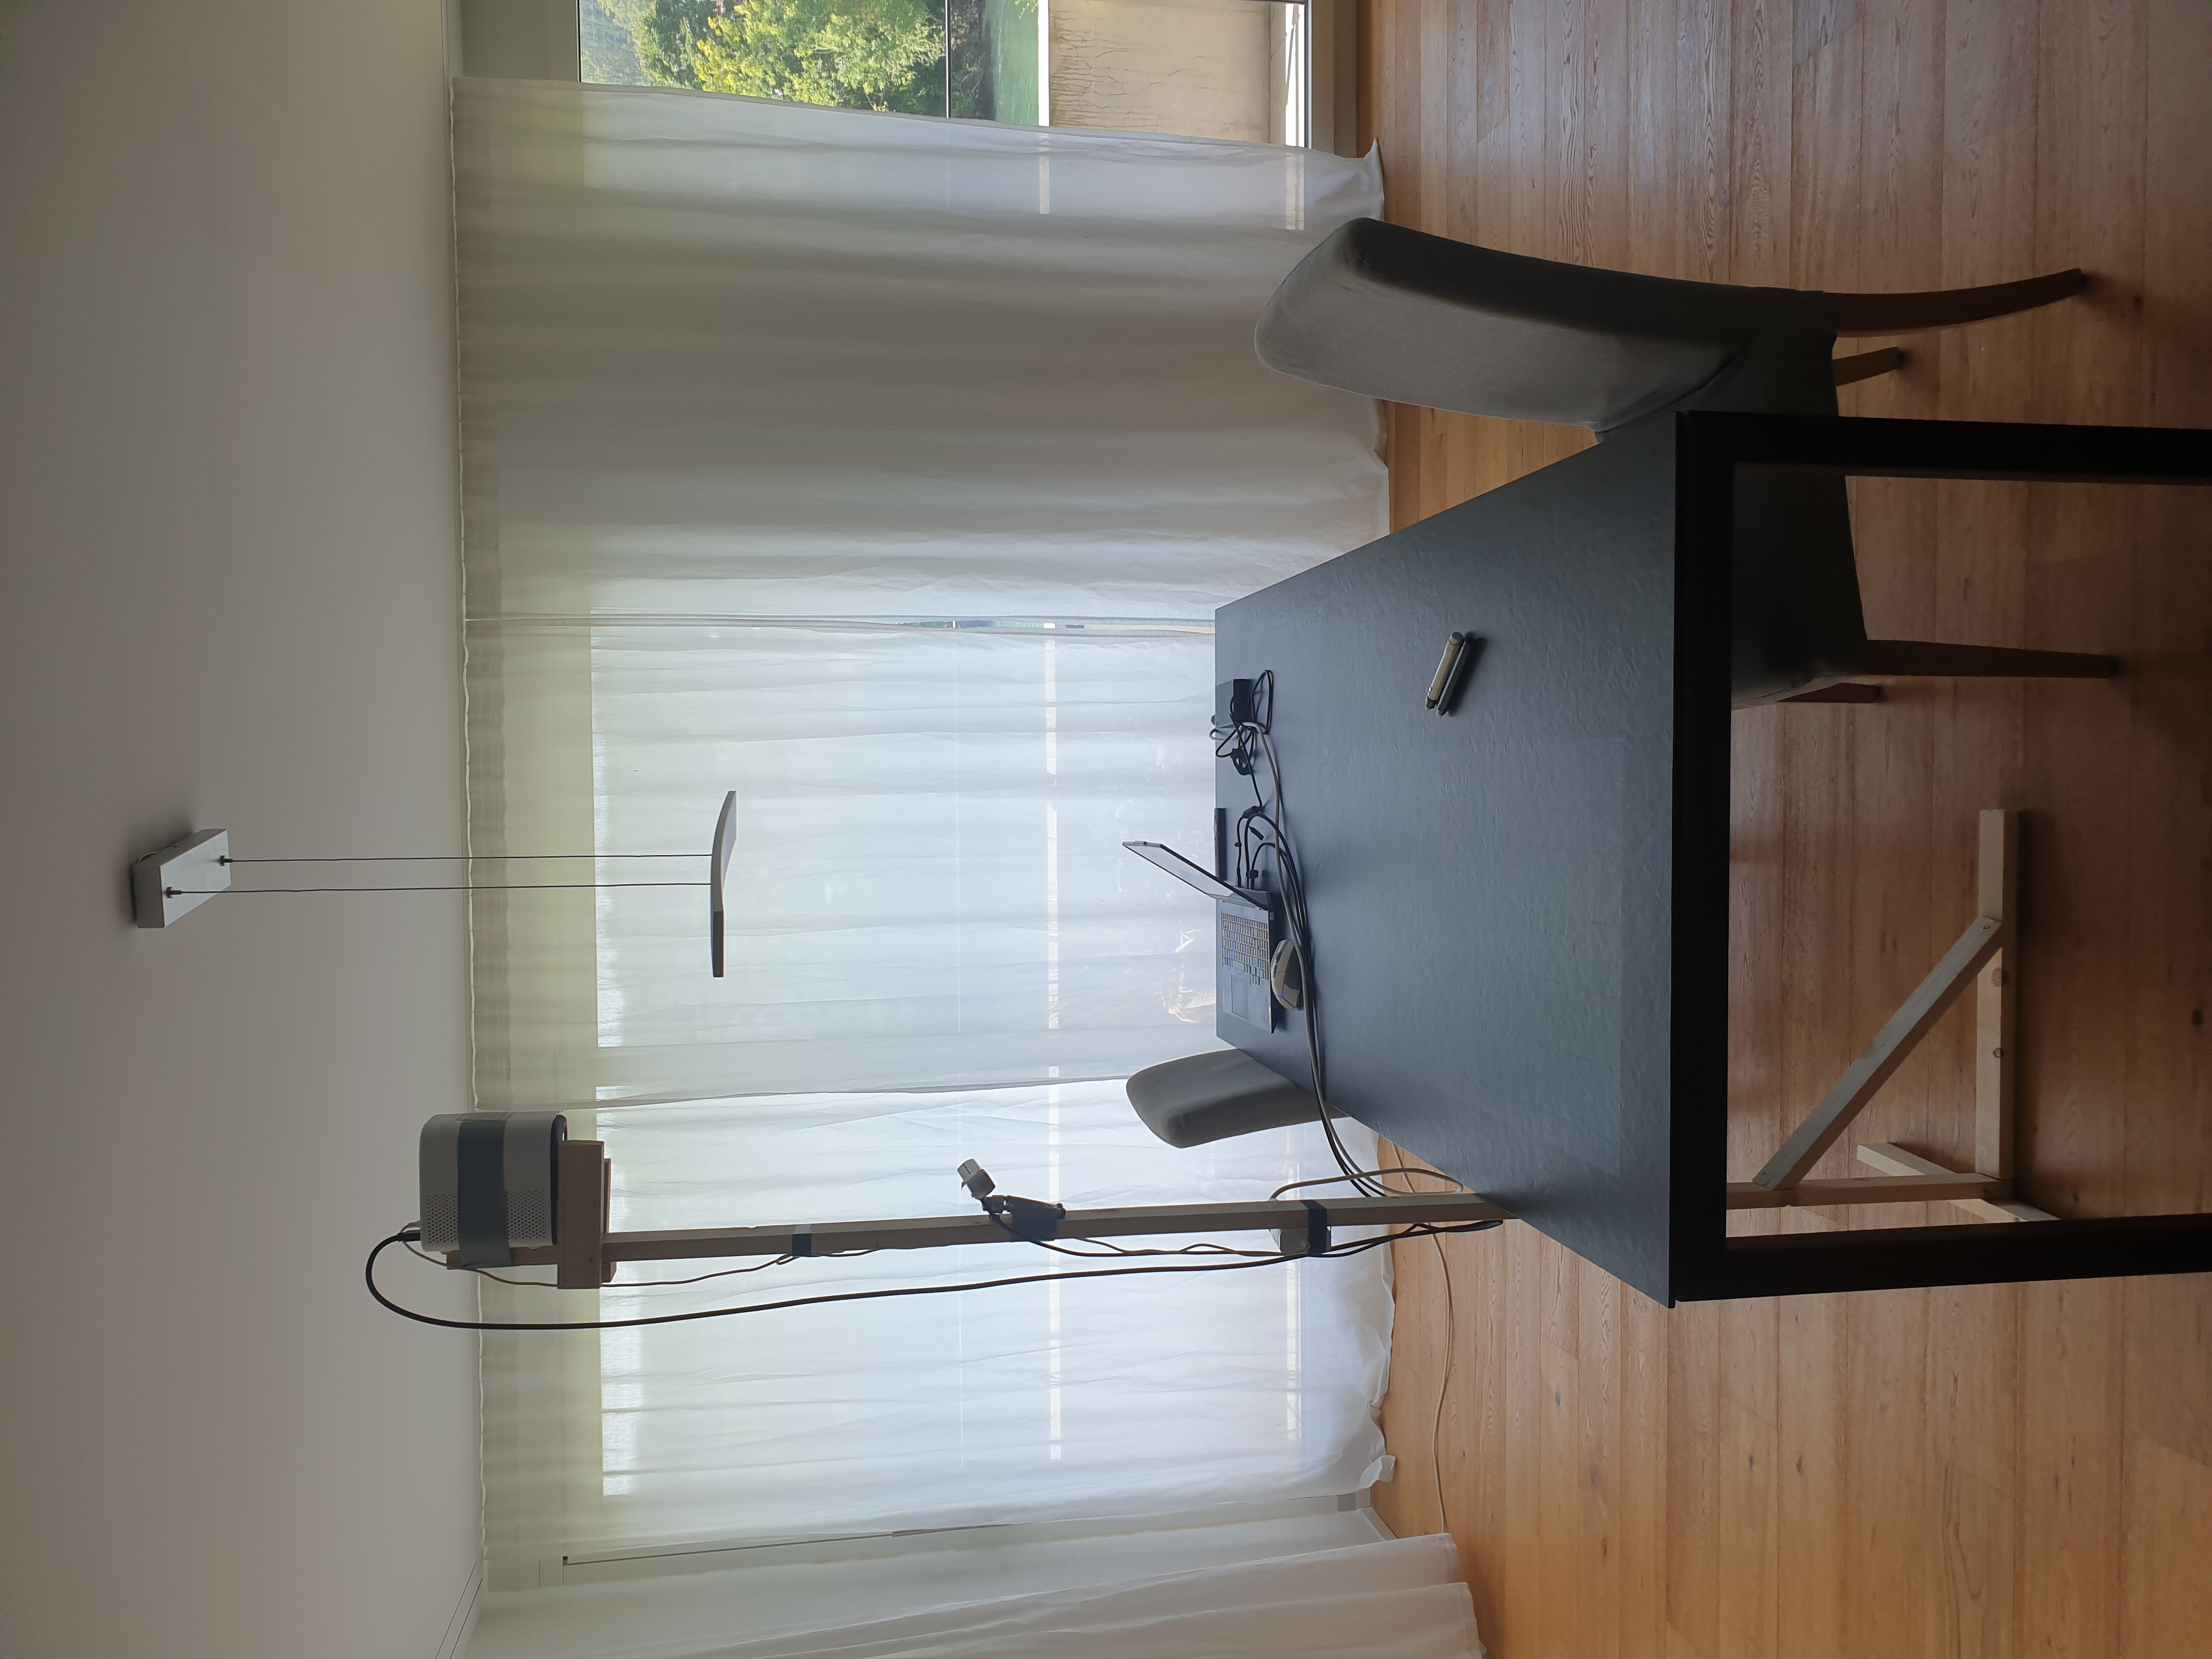
\includegraphics[width=0.7\linewidth, angle=-90]{graphics/sus_setup_2.jpg}}
    \caption{Gesamtansicht der Testumgebung (SUS)}
    \label{Fig:Data2}
  \end{minipage}
\end{figure}


\subsection{SUS-Auswertung}

Zur Bewertung der Gebrauchstauglichkeit wurde die etablierte Methode des \textit{System Usability Scale} (SUS) verwendet. Der SUS ist ein standardisiertes Umfrageinstrument, das aus zehn Aussagen besteht, die von den Teilnehmenden auf einer fünfstufigen Likert-Skala (von „stimme überhaupt nicht zu“ bis „stimme voll und ganz zu“) bewertet werden. Der SUS ist bewusst allgemein gehalten, um auf unterschiedlichste digitale Systeme angewendet werden zu können. Er erfasst sowohl die wahrgenommene Einfachheit als auch die Effizienz der Nutzung und erlaubt einen Vergleich mit anderen Systemen anhand eines normierten Scores. Ein Mittelwert von 68 gilt dabei als durchschnittliche Usability. Im Rahmen des Tests mit vier Teilnehmenden wurde der SUS nach Abschluss der praktischen Erprobung der Anwendung ausgefüllt. Die Ergebnisse wurden anschliessend mithilfe einer standardisierten Template-Berechnung ausgewertet, bei der jedem Item ein Punktewert zugeordnet und auf eine Skala von 0 bis 100 normiert wird. Diese Vorgehensweise bietet eine einfache und zugleich wissenschaftlich etablierte Möglichkeit, die wahrgenommene Benutzerfreundlichkeit zu quantifizieren. Sie eignet sich insbesondere für kleinere Testgruppen und liefert dennoch verlässliche Aussagen über die grundsätzliche Akzeptanz und Bedienbarkeit eines Systems.\\  \cite{brooke1986sus} \cite{uiuxtrendSUS}

Die Bewertungen ergaben folgende Scores:
\begin{itemize}
    \item \textbf{Person 1:} 67.5 Punkte
    \item \textbf{Person 2:} 85.0 Punkte
    \item \textbf{Person 3:} 75.0 Punkte
    \item \textbf{Person 4:} 70.0 Punkte
    \item \textbf{Person 5:} 87.5 Punkte
    \item \textbf{Person 6:} 85.0 Punkte
\end{itemize}

Der Mittelwert liegt bei \textbf{78.33 Punkten}. Dies weist auf eine insgesamt gute bis sehr gute Gebrauchstauglichkeit der Anwendung hin. Abbildung~\ref{fig:sus_scores_updated_v2} visualisiert die Ergebnisse im Vergleich zum Standardbenchmark.

\begin{figure}[H]
    \centering
    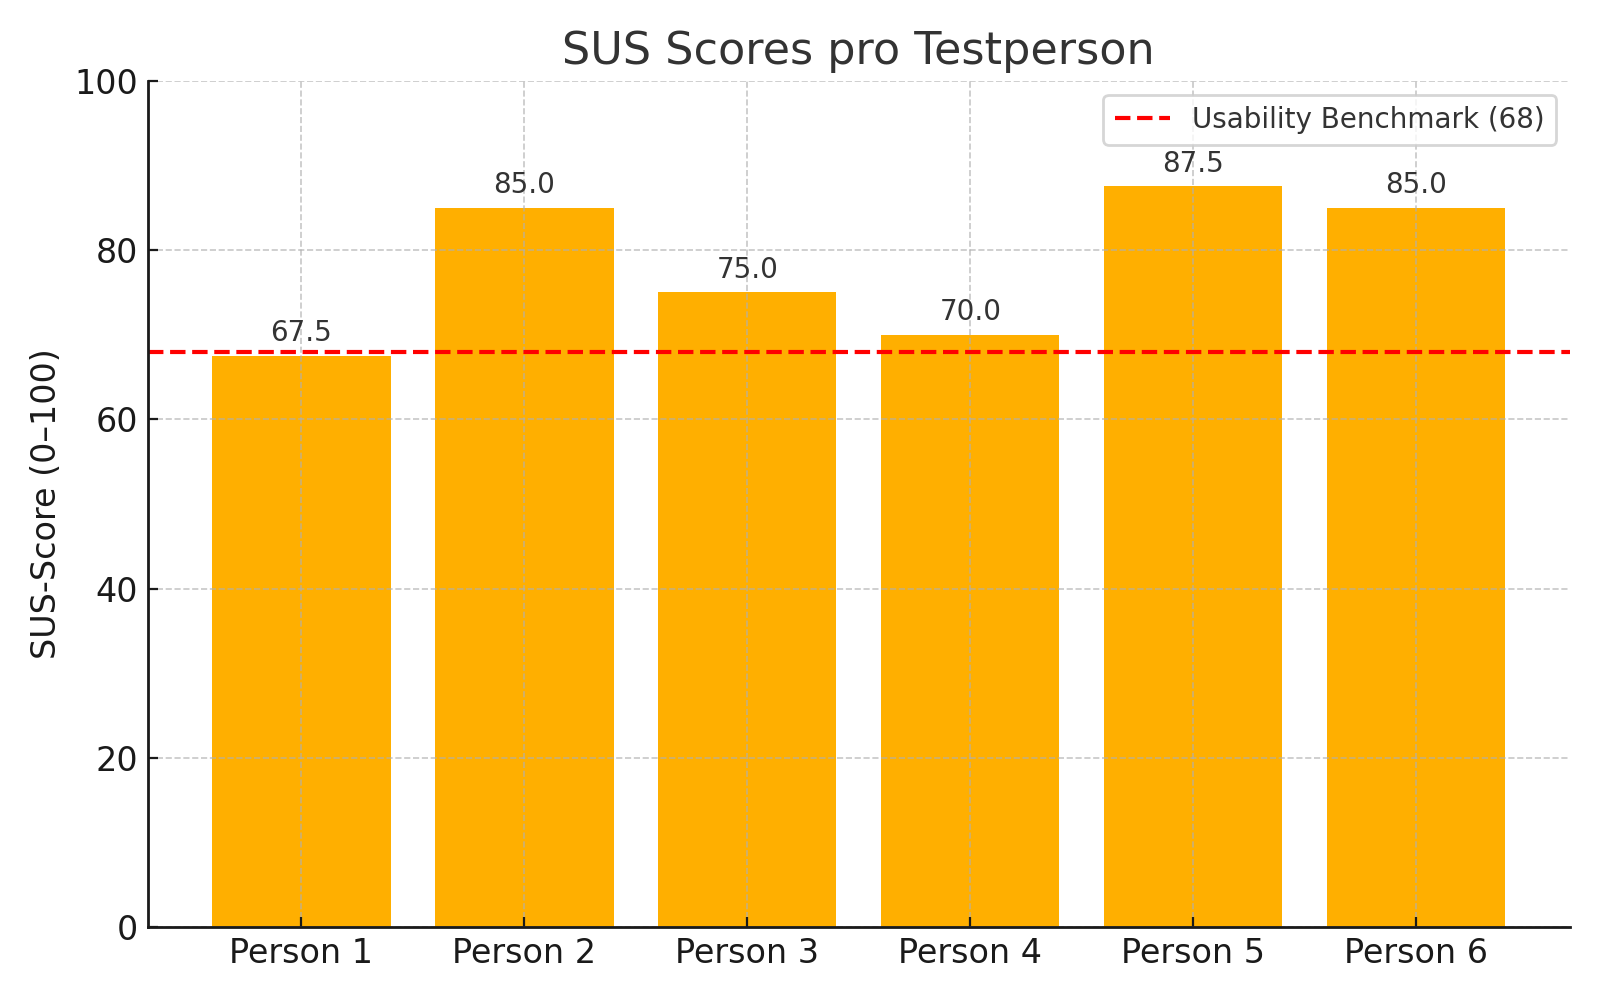
\includegraphics[width=0.65\textwidth]{graphics/sus_scores_plot.png}
    \caption{SUS-Bewertung aller Testpersonen im Vergleich zum Benchmark (68 Punkte)}
    \label{fig:sus_scores_updated_v2}
\end{figure}

\clearpage

\subsection{Qualitatives Feedback und Beobachtungen}

Neben der quantitativen Bewertung wurde zusätzlich qualitatives Feedback in Form von offenen Fragen und Beobachtungen erhoben. Dieses qualitative Feedback ermöglicht eine vertiefte Analyse und liefert detaillierte Einblicke in die Stärken und Schwächen der Anwendung. Dadurch können nicht nur allgemeine Tendenzen, sondern auch spezifische Verbesserungspotenziale identifiziert werden, die in der quantitativen Auswertung möglicherweise nicht erkennbar sind.


\textbf{Positiv bewertet wurden:}
\begin{itemize}
    \item Das grundlegende Konzept wurde mehrfach positiv beurteilt. Insbesondere das freie Zeichnen auf einer beliebigen Zeichenfläche kam bei fast allen Testpersonen sehr gut an.
    \item Die einfache und intuitive Bedienung wurde durchgehend als positiv empfunden.
\end{itemize}

\textbf{Herausforderungen und Verbesserungspotenziale:}
\begin{itemize}
    \item Es herrschte Unsicherheit bezüglich der Bedeutung einzelner Icons. So wurde beispielsweise das Rotations-Icon von mehreren Testpersonen fälschlicherweise als „Undo“-Button interpretiert.
    \item Bei einigen Tests traten noch Bugs sowie Präzisionsprobleme auf, welche negativ auffielen.
    \item Die Radierfunktion erhielt gemischtes Feedback. Einige Nutzer wünschten sich mehr Auswahlmöglichkeiten bezüglich der Funktionsweise. Insbesondere wurde kritisiert, dass der Hintergrund mitgelöscht wird. Dies wurde von einigen Personen negativ bewertet, während andere die Funktion grundsätzlich akzeptierten, jedoch einen separaten Modus forderten, um Striche oder Bereiche zu löschen, ohne den Hintergrund zu beeinträchtigen.
\end{itemize}



Grundsätzlich wurden vor allem fehlende Funktionen sowie Funktionen mit unzureichendem Umfang negativ bewertet, während die Qualität und Verständlichkeit insgesamt als gut eingeschätzt wurden. Das qualitative Feedback und die Beobachtungen erwiesen sich dabei als besonders wertvoller Input. So wurde beispielsweise bereits bei der ersten Testperson festgestellt, dass das ursprüngliche Konzept für ein Setup mit einer Kamera im 90°-Winkel zur Zeichenfläche nicht optimal ist. Dieses Problem konnte daraufhin unmittelbar behoben werden, sodass es bei allen nachfolgenden Tests nicht mehr auftrat.
\clearpage

\subsection{Feldtest mit Kundeninterview}

Um das Verhalten des Systems in einer möglichst realitätsnahen Umgebung zu prüfen, wurde ein Feldtest direkt beim SCDH in Nidau durchgeführt. 
Dabei wurde das System vor Ort installiert und im Rahmen einer Demonstration für den SCDH ein simulierter Workshopablauf durchgespielt. 
Anschliessend wurde ein Interview mit David Wollschlegel geführt, um seine Einschätzung zum System einzuholen. 
Dabei wurden verschiedene Punkte zum System, zu den Integrationsmöglichkeiten sowie zu Verbesserungs- und Erweiterungspotenzialen erörtert. 
Insgesamt zeigte sich David Wollschlegel sehr zufrieden mit dem Endstand des Projekts.


\begin{figure}[H]
    \centering
    \includegraphics[width=0.65\linewidth]{graphics/übersicht_feldtest.JPG}
    \caption{Setup beim Feldtest im SCDH}
    \label{fig:placeholder}
\end{figure}

\textbf{Positive Punkte:}
\begin{itemize}
    \item Das System erfüllt grundsätzlich die gestellten Anforderungen.
    \item Es fügt sich bereits gut in die bestehenden Arbeitsprozesse des SCDH ein.
    \item Insgesamt weist es ein vielversprechendes Potenzial auf und bietet einen klaren Mehrwert gegenüber bestehenden Methoden und Möglichkeiten.
\end{itemize}

\textbf{Negative Punkte:}
\begin{itemize}
    \item Ein leichter Offset wurde als geringfügig störend wahrgenommen, jedoch nicht als gravierend bewertet.
\end{itemize}

\textbf{Feedback zur Zukunft:}
\begin{itemize}
    \item Mögliche Hürden bei der Einführung in ein produktives Umfeld am SCDH liegen nicht im System selbst, sondern in der Beschaffung, dem Setup vor Ort sowie der Integration in die bestehende Softwarelandschaft des SCDH.
    \item Das System bietet dem SCDH die Möglichkeit, neue Angebote zu entwickeln.
    \item Es wurden verschiedene Feature-Wünsche und Ideen besprochen, beispielsweise ein Objektkatalog, Cloud- und Remote-Funktionen sowie weitere Features und \emph{Quality-of-Life}-Verbesserungen.
\end{itemize}


\begin{figure}[H]
    \centering
    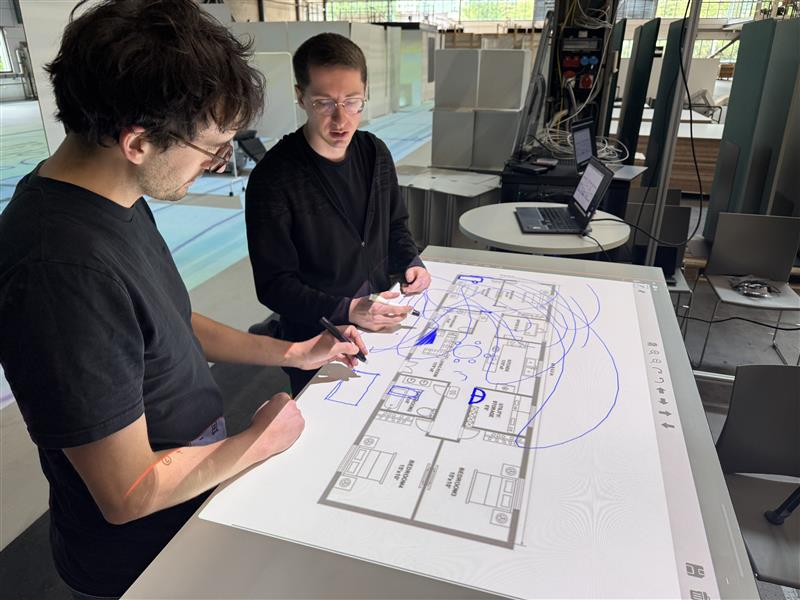
\includegraphics[width=0.65\textwidth]{graphics/feldtest.JPG}
    \caption{Feldtest am SCDH mit dem Kunden}
    \label{fig:feldtest}
\end{figure}

\subsection{Fazit}

Die Tests zeigten, dass die Anwendung sehr gut angenommen wird. Der durchschnittliche SUS-Wert liegt mit 78.33 Punkten deutlich über dem branchenüblichen Schwellenwert von 68 Punkten und bestätigt damit eine hohe Gebrauchstauglichkeit.  
Da die Bewertung nach der anerkannten \textit{System Usability Scale} (SUS) erfolgte, sind die Ergebnisse gut mit anderen Studien und Systemen vergleichbar und unterstreichen die methodische Validität der Erhebung.  

Neben den positiven quantitativen Ergebnissen lieferten auch die qualitativen Rückmeldungen wertvolle Hinweise für mögliche Optimierungen. Der durchgeführte Feldtest mit dem Kunden bestätigte die Praxistauglichkeit der Lösung und identifizierte zentrale Verbesserungspotenziale wie eine optimierte Kalibrierung, zusätzliche Funktionen wie Undo/Redo sowie erweiterte Integrationsmöglichkeiten.  

Insgesamt steht fest, dass die entwickelte Lösung sowohl in ihrer aktuellen Form produktiv eingesetzt werden kann als auch eine solide Basis für zukünftige Erweiterungen bietet. Der erzielte Entwicklungsstand erfüllt die gesteckten Projektziele vollständig und belegt das Potenzial des Systems für den langfristigen Einsatz in unterschiedlichen Anwendungskontexten.


